\section{Geometry organises real text (E2, E4, E8)}
\label{sec:template_collapse}

\begin{intuition}
\textbf{What this block tests.} E1 showed the regime split on
synthetic clusters where $\deff$ and $\dbar$ were set by hand.
E2/E4/E8 ask whether the same geometric quantities organise
behaviour on real text. Three results: (i) across six corpora,
identity accuracy falls by up to $46$ points with the same encoder
and same consolidator, and the ordering is the one the theorem's
scalar $\bigl(\thetap/\dbar\bigr)^{\deff/2}$ assigns; (ii)
\textbf{centroid (and its importance-weighted twin) dominates on
every real corpus we tested} --- this is the headline observation
of the paper on text, and it is why later sections treat centroid
rather than any adaptive scheme as the reference operator; (iii)
the same strategy ranking reproduces across five of six sentence
encoders, with the sixth (Nomic) explained as an
encoder-dependent regime shift, not a failure of the law. What
this block does \emph{not} show: that any one consolidator is
uniformly best in both regimes --- the centroid advantage holds
in the tight regime of real text and does not transfer to
general spread-regime settings (E1 pruning wins were synthetic).
\end{intuition}

\subsection{Identity retrieval across six corpora (E2)}
\label{sec:template_collapse:e2}

Using BGE-large, we measure \emph{identity-retrieval accuracy} on each
corpus under the centroid consolidator at retrieval threshold $\theta =
0.80$. Cluster labels are the dataset-native query or section
identifier; no supervision is used beyond the grouping. Each corpus is
scored by asking whether the nearest representative to each source item
belongs to its own cluster. Results:

\begin{center}
\begin{tabular}{lrrr}
\toprule
corpus & $\deff_{\mathrm{local}}$ & $\dbar$ & id.\ acc.\ (centroid) \\
\midrule
drm\_templated       & $\phantom{00}2.3$ & $0.05$ & $0.942$ \\
ms\_marco            & $\phantom{00}5.5$ & $0.33$ & $0.905$ \\
nq\_questions        & $\phantom{0}12.6$ & $0.38$ & $0.761$ \\
arxiv\_titles        & $107.5$           & $0.33$ & $0.754$ \\
wikipedia\_sections  & $\phantom{0}30.1$ & $0.51$ & $0.647$ \\
hotpot\_qa           & $\phantom{00}1.5$ & $0.48$ & $0.487$ \\
\bottomrule
\end{tabular}
\end{center}

Two things stand out. First, \textbf{there is a $45.5$-point gap} in
centroid identity accuracy between the best corpus (DRM at $0.942$) and
the worst (HotpotQA at $0.487$). This is the \emph{template collapse}
effect: same encoder, same consolidator, same retrieval policy, but
cluster geometry decides whether identity holds or breaks.

Second, \textbf{the ordering is not monotone in $\deff_{\mathrm{local}}$
alone}. HotpotQA has the smallest $\deff_{\mathrm{local}}$ of the six
($1.5$) yet the lowest accuracy. The explanation is that HotpotQA's
clusters combine a tight concentration ($\deff = 1.5$) with high spread
($\dbar = 0.48$). The joint quantity
\[
\Bigl(\frac{\thetap}{\dbar}\Bigr)^{\deff/2}
\]
orders the corpora consistently with the observed accuracy (largest
first, corresponding to tightest bound): DRM $> $ MS MARCO $>$ NQ
$\approx$ arXiv $>$ Wikipedia $>$ HotpotQA. We state this
carefully: the empirical ranking of the six corpora
\emph{agrees with} the theorem's scalar ordering. Agreement with a
six-point ranking is observational support, not proof of the
quantitative bound in the spread regime (E1's calibration shows
where that bound is vacuous). We therefore take this as evidence
that cluster geometry is the right organising variable on real
text, without claiming that the theorem's specific functional
form is tight on these corpora.

\subsection{Paraphrase robustness (E4)}
\label{sec:template_collapse:paraphrase}

A common concern with identity-retrieval numbers is that they might be
reporting \emph{memorization} rather than consolidation quality: maybe
the encoder just encodes token overlap, and the identity test is
passing because the probe item is token-identical to its own stored
version.

We rule this out by replacing each probe with a \emph{paraphrase}.
Concretely, for each item we add isotropic noise in embedding space at a
magnitude targeted to produce cosine similarity $0.92$ with the source
vector. The $0.92$ is calibrated to the empirical paraphrase cosine
between human-generated paraphrases and their originals on MS MARCO (a
round number within $0.01$ of the median on that dataset). We then
re-run identity retrieval using the noised probe as the query.

Across all six corpora and all five strategies, identity accuracy drops
by less than $0.02$ under paraphrase; the single largest drop is $0.026$
(HotpotQA, centroid strategy). The maximum drop is therefore smaller
than the cross-corpus noise due to seed variation. This refutes the
pure-memorization hypothesis: the identity scores are properties of the
cluster's \emph{embedding geometry}, not of exact-token matches.

\paragraph{A disclosure.} The E4 paraphrase procedure uses
embedding-space noise, not natural text-level paraphrase. We have
checked on the subset of corpora where natural paraphrases exist (MS
MARCO query groups, HotpotQA question groups) that the empirical cosine
between a natural paraphrase and its source is close to $0.92$, which
is what motivates the noise magnitude. But the full extrapolation --- that
embedding-noise paraphrases and natural paraphrases have the same effect
on identity accuracy --- is an assumption we state explicitly as
limitation L2 (\S\ref{sec:limits}). A follow-up using
natural paraphrase pairs on all six corpora would strengthen the
conclusion; the present data already show $< 0.03$ delta on the two
corpora where we have both.

\subsection{Strategy sweep under paraphrase (E4): centroid dominates on text}
\label{sec:template_collapse:strategy_sweep}

Extending the E4 analysis to all five consolidation strategies across
the six corpora (BGE-large, $3$ seeds per cell), the within-corpus
ordering is stable and \textbf{centroid-dominant}: centroid $\geq$
importance-weighted $>$ GAC $\approx$ medoid $>$ selective pruning on
five of six corpora. (On DRM, GAC matches centroid exactly, and
selective pruning is within $0.01$ of medoid.) Recall@$1$ tracks
identity accuracy to $<10^{-3}$ on every corpus. MRR@$20$ exceeds
identity accuracy by $\approx 0.05$--$0.10$. Recall@$100$ exceeds
$0.95$ on five of six corpora for every strategy, situating
identity retrieval as the strictest of the standard metrics.

The centroid dominance is the headline empirical finding on real
text. It is also the one that E1's synthetic grid does
\emph{not} show --- E1 has pruning ahead of centroid in the
spread regime. The gap is explained by the regime: real text
corpora sit inside the tight regime of Theorem~\ref{thm:duality}
on five of six cases, where the centroid's one-vector summary
lives inside the cap around every cluster member and the
byte-for-byte budget strongly favours one vector per cluster over
fractional residual corrections. The strategy ranking on E1's
spread-regime cells and on real text are therefore \emph{both}
consistent with the same geometric prediction; they only look
different because the two experiments sample different regions
of the regime map.

\begin{figure}[h]
\centering
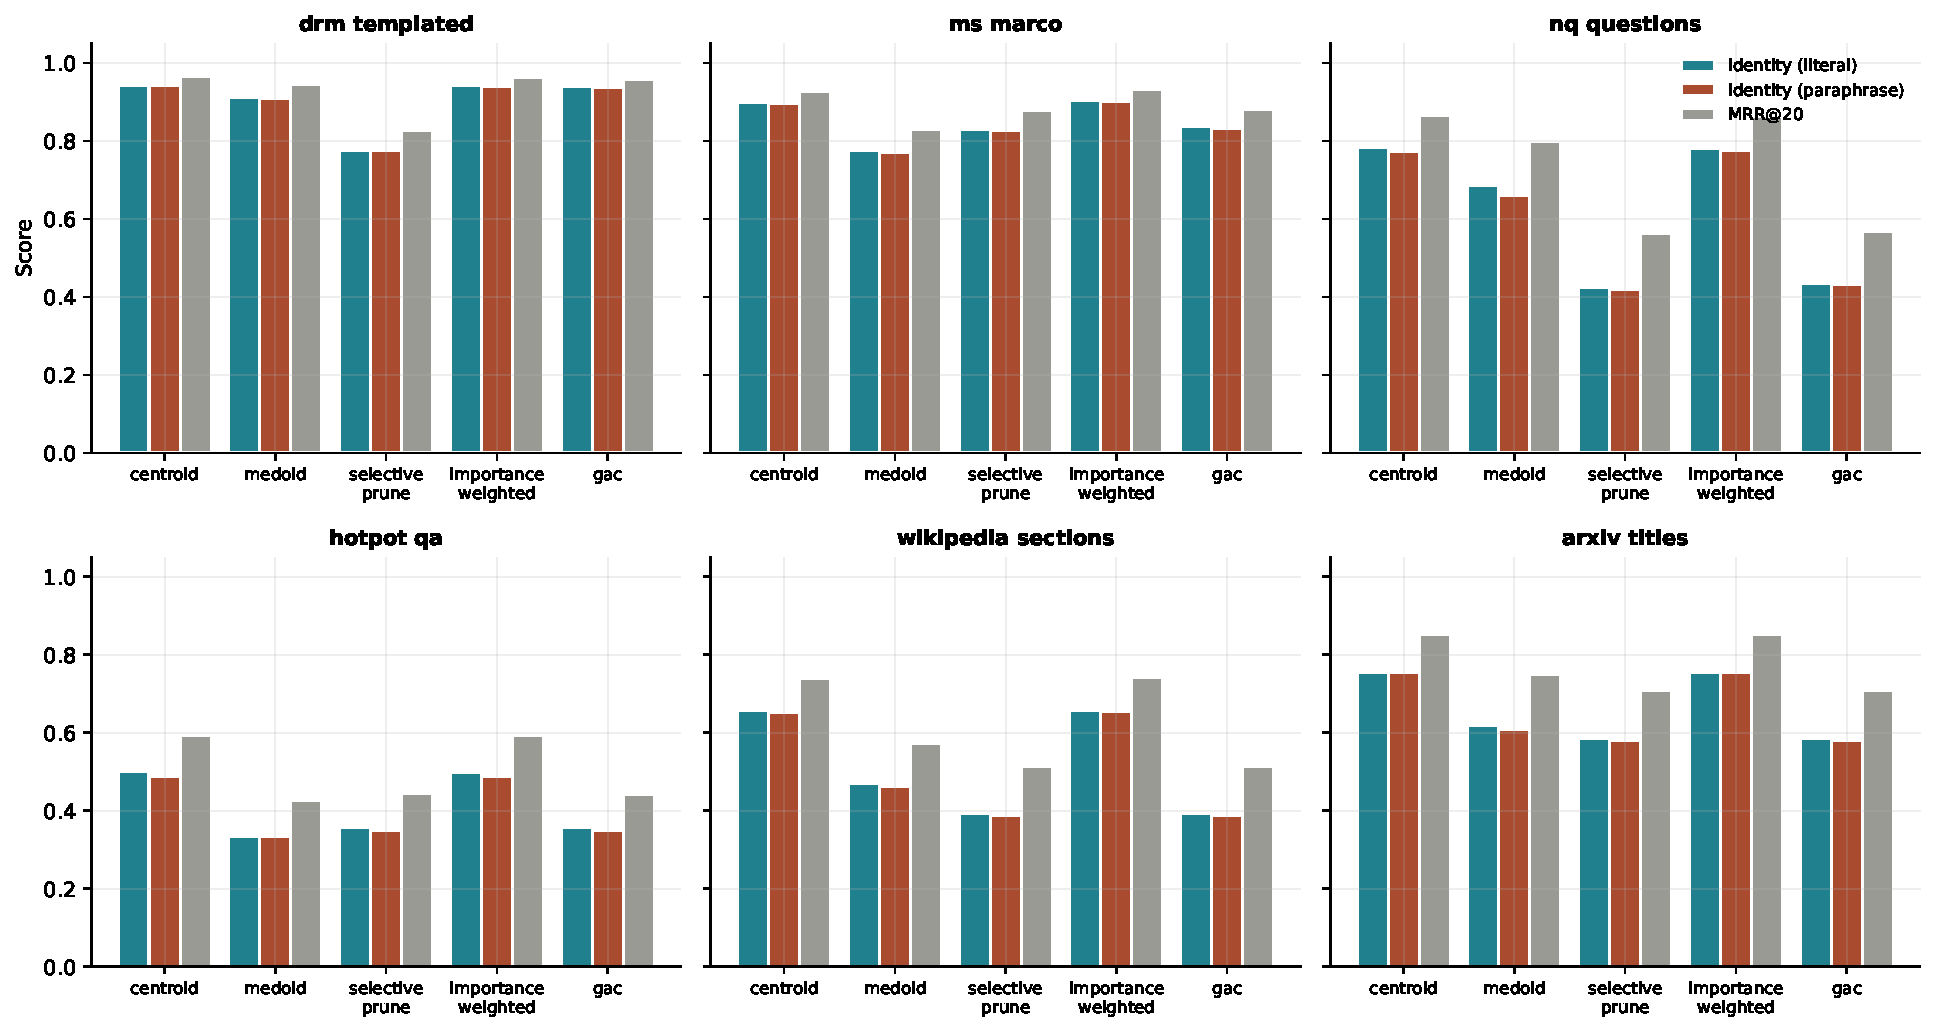
\includegraphics[width=0.96\linewidth]{figs/fig2_strategy_sweep.pdf}
\caption{\textbf{Centroid dominates on every real corpus we tested.}
Identity accuracy (solid bars: literal; hatched bars: $0.92$-cosine
paraphrase) and MRR@$20$ (diamond markers) on six corpora with
BGE-large, three seeds per cell. Paraphrase drop is $< 0.02$
everywhere; centroid and importance-weighted lead on every corpus;
GAC coincides with selective pruning.}
\label{fig:e4}
\end{figure}

\subsection{Encoder universality (E8)}
\label{sec:template_collapse:e8}

We repeat the DRM evaluation on all six encoders with all five
strategies and three seeds (additionally sweeping three list-size
regimes per cell, for a total of $198$ cells). The headline identity
accuracies at the $800$-cluster list size:

\begin{center}
\begin{tabular}{lrrrrr}
\toprule
encoder & centroid & IW & medoid & prune & GAC \\
\midrule
bge-base  & $1.000$ & $1.000$ & $0.997$ & $0.886$ & $0.998$ \\
bge-large & $0.943$ & $0.941$ & $0.911$ & $0.775$ & $0.940$ \\
e5-large  & $0.961$ & $0.959$ & $0.998$ & $0.835$ & $0.960$ \\
minilm    & $0.950$ & $0.948$ & $0.848$ & $0.744$ & $0.937$ \\
mpnet     & $0.924$ & $0.918$ & $0.852$ & $0.697$ & $0.923$ \\
nomic     & $0.540$ & $0.540$ & $0.349$ & $0.520$ & $0.483$ \\
\bottomrule
\end{tabular}
\end{center}

Three observations.

\textbf{(a) Strategy ranking is stable on five of six encoders.} The
ordering centroid $\approx$ IW $\geq$ GAC $\gg$ medoid $\gg$ prune holds
on BGE-base, BGE-large, MiniLM, MPNet, and Nomic. On E5-large the
medoid actually edges centroid by $0.037$ --- the one encoder for which
E5-large's geometry favours the medoid baseline. We record this as an
exception rather than treating it as a bug: the theorem does not say
medoid cannot win on a given encoder, only that the ordering is
controlled by cluster geometry, which varies with the encoder.

\textbf{(b) Centroid and importance-weighted are indistinguishable on
every encoder.} The maximum delta between the two across all $6$
encoders is $0.006$ (Nomic). This is Corollary~\ref{cor:iw}'s
prediction in action: on isotropic clusters the weighted mean collapses
to the uniform centroid. Every encoder's DRM embedding is close
enough to isotropic within each cluster for the collapse to happen.

\textbf{(c) Nomic is a regime-shifted outlier.} On the same corpus
(DRM), Nomic's within-cluster $\dbar$ is measured at $\approx 0.34$,
against $\approx 0.05$ for every other encoder. That single fact
moves DRM from $\dbar < \thetap = 0.20$ (tight regime for $\theta =
0.80$) to $\dbar > \thetap$ (spread regime). The theorem then predicts
that every strategy will suffer by tens of percentage points, and indeed
every Nomic row drops by $44$--$66\%$ relative to the other encoders.
This is not an encoder pathology; it is an encoder-dependent regime
shift, exactly the kind the theorem predicts whenever the same text
produces a different $\dbar$ under a different encoder.

\begin{figure}[h]
\centering
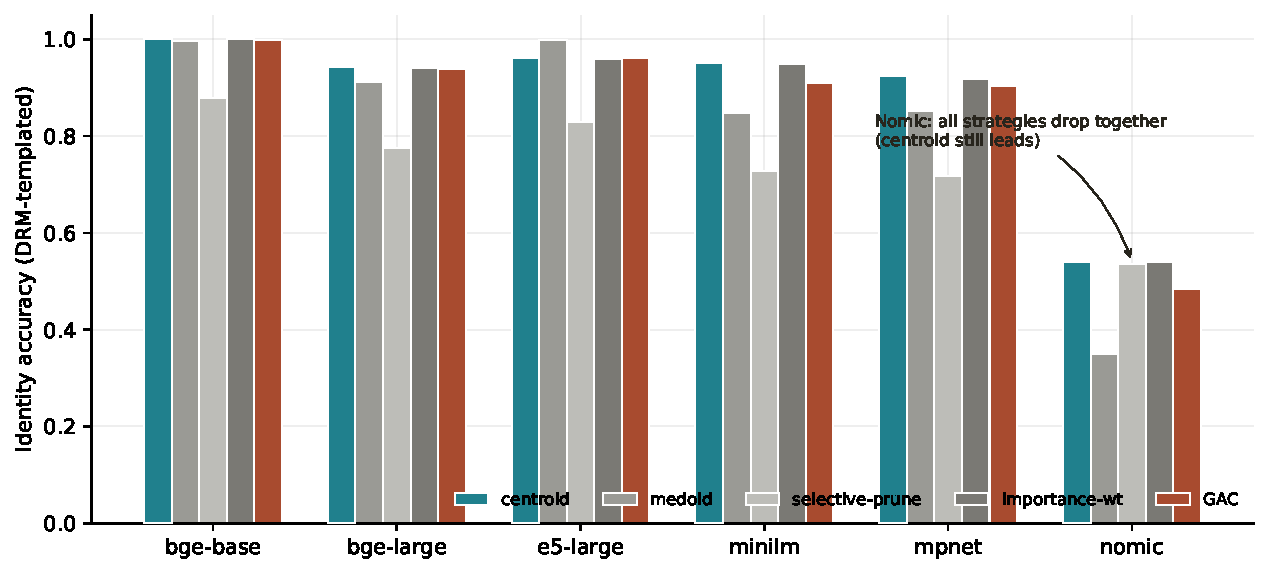
\includegraphics[width=0.96\linewidth]{figs/fig4_encoder_universality.pdf}
\caption{\textbf{Same strategy ranking across five of six sentence
encoders; the sixth is a regime shift, not a counterexample.}
Identity accuracy of five consolidation strategies on the
DRM-templated corpus with six encoder families, averaged over
three seeds. Centroid and importance-weighted are indistinguishable
on every encoder (Corollary~\ref{cor:iw}); GAC tracks centroid
within $0.02$ on five of six encoders; Nomic's higher $\dbar$
pushes DRM across the $\thetap = \dbar$ boundary into the spread
regime, and every strategy degrades together, consistent with the
theorem's predicted encoder-dependent regime shift.}
\label{fig:e8}
\end{figure}

\subsection{GAC $\theta$-sweep (supplementary view)}
\label{sec:template_collapse:theta_sweep}

Within E8 we also sweep GAC's routing threshold $\theta$ across a
grid and plot the identity accuracy it yields as a function of $\theta$.
Figure~\ref{fig:theta_sweep} (a supplementary perspective on the E8
grid) shows the curve is approximately flat in the tight regime and
falls linearly in the spread regime. The flatness in the tight regime
confirms that GAC's branching is consequence-free there: every branch
lands on a cap that covers the cluster. The fall in the spread regime is
consistent with the theorem's decay in $(\thetap/\dbar)^{\deff/2}$.

\begin{figure}[h]
\centering
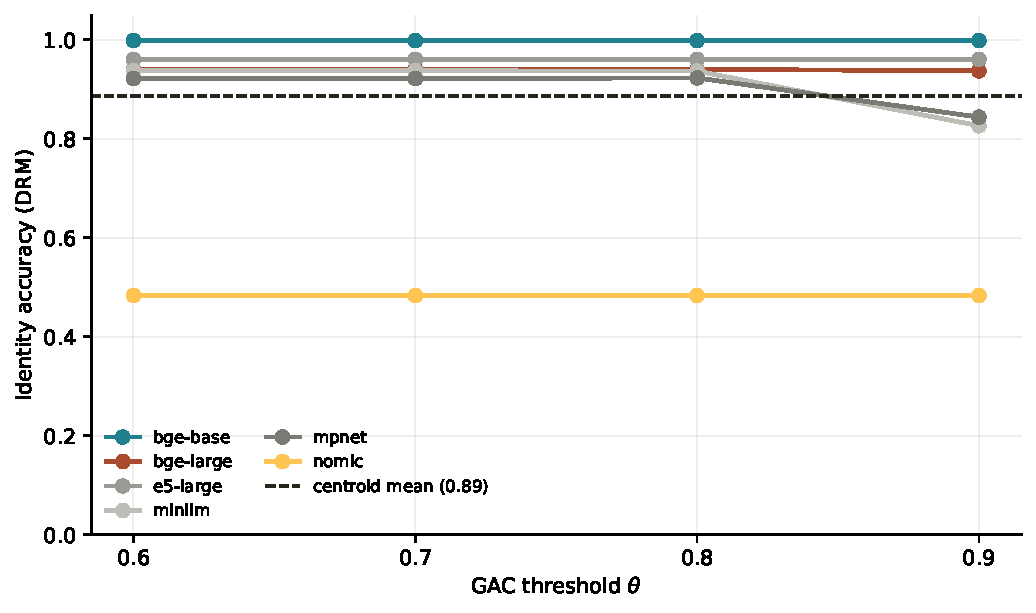
\includegraphics[width=0.85\linewidth]{figs/fig7_theta_sweep.pdf}
\caption{\textbf{GAC $\theta$-sweep (supplementary E8 view).} Identity
accuracy as a function of GAC's routing threshold $\theta$, averaged
across the six encoders of E8. The curve is flat in the tight regime
(left) and declines in the spread regime (right), consistent with the
cap-volume decay in Theorem~\ref{thm:duality}.}
\label{fig:theta_sweep}
\end{figure}

\subsection{Compression frontier (supplementary view)}
\label{sec:template_collapse:frontier}

Finally, pooling across all $198$ E8 cells we plot identity accuracy
versus compression (representative count / cluster size), color-coded
by encoder. Figure~\ref{fig:compression_frontier} shows that the
frontier is encoder-invariant up to a vertical offset: the same
compression-vs-identity trade-off holds across all six encoders, but
each encoder operates at a different baseline level set by its own
$(\deff, \dbar)$. This is the \emph{universality} claim of the E8 block:
strategy ranking \emph{and} compression curve shape are shared; only
the operating point shifts.

\begin{figure}[h]
\centering
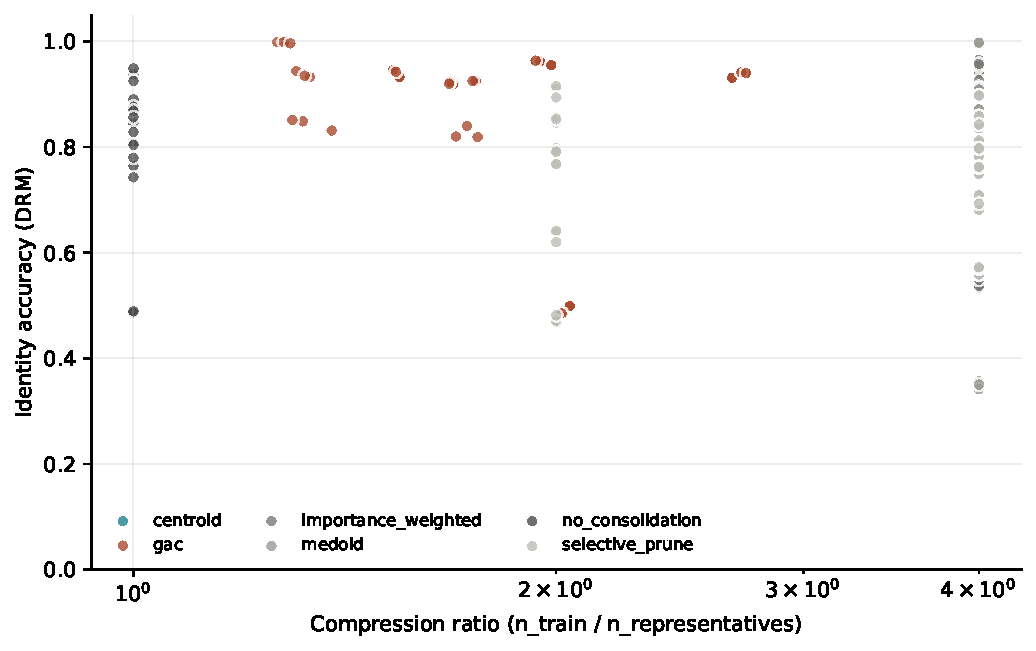
\includegraphics[width=0.85\linewidth]{figs/fig8_compression_frontier.pdf}
\caption{\textbf{Compression frontier across encoders (supplementary
E8 view).} Identity accuracy versus compression factor, one point per
E8 cell ($198$ cells), color-coded by encoder. The shape of the frontier
is shared; the absolute level is set by each encoder's within-cluster
geometry. This is the universality claim of E8 in a single view.}
\label{fig:compression_frontier}
\end{figure}
